\documentclass[../main.tex]{subfiles}

\begin{document}
\begin{flushleft} 
\section{Design}

%Indledning af design-afsnittet
\TODO Intro tekst
I designfasen af projektet vil der tages udgangspunkt i de stillede designmæssige krav til at lave bræspillet. De krav der er sat. og som vil blive udarbejde. er til at vise vores bruge af GRASP principperne, lave et designklassediagram, lave et sekvensdiagram og (muligvis) lave et pakkediagram. 


%Indledning til GRASP-principper
\subsection{GRASP (!Indsat kopi fra CDIO-2!)}
\TODO[Må vi kopiere denne del fra CDIO-2? Ellers skal dette omskrives]

Vi vil benytte GRASP principperne til at designe vores diagrammer, således at software-klasserne har et veldefineret og afgrænset ansvar som understøtter reusability. \newline

\vspace{5mm}
De følgende GRASP principper forklares og argumenteres for under designklassediagrammet:
\begin{itemize}
    \item Creator: Ansvar for objektskabelse
    \item Information Expert: Ansvar for tildeling af ansvar til objekter
    \item Low Coupling: Ansvar for lav afhængighed/associationer mellem klasserne
    \item High Cohesion: Ansvar for høj samhørighed mellem klasserne
    \item Controller: Ansvar for input til systemet
\end{itemize}



%Designklassediagram
\subsection{Designklassediagram (!Indsat kopi fra CDIO-2!)}
\TODO[Må vi kopiere denne del fra CDIO-2? Ellers skal dette omskrives]

Et designklassediagram laves på baggrund af GRASP-principperne samt tidligere analytiske arbejde med særligt udgangspunkt i  vores domænemodel (Figur \ref{fig:domain}), som indeholder concepter af klasser. I designklassediagrammet arbejder vi med software-klasser, som skal implementeres i systemet. Her har software-klasserne mere konkrete beskrivelser end domænemodellen. Derfor er der bl.a. beskrevet attributter, tilhørende metoder og relationer mellem klasserne. Designklassediagrammet arbejdes dermed også videre på i implementationsfasen, da der vil opstå ændringer undervejs. Understående diagram er vores endelige dokumenterede designklassediagram for systemet:


%Designklassediagram
\begin{figure}[H]
    \centering
    \rotatebox{270}{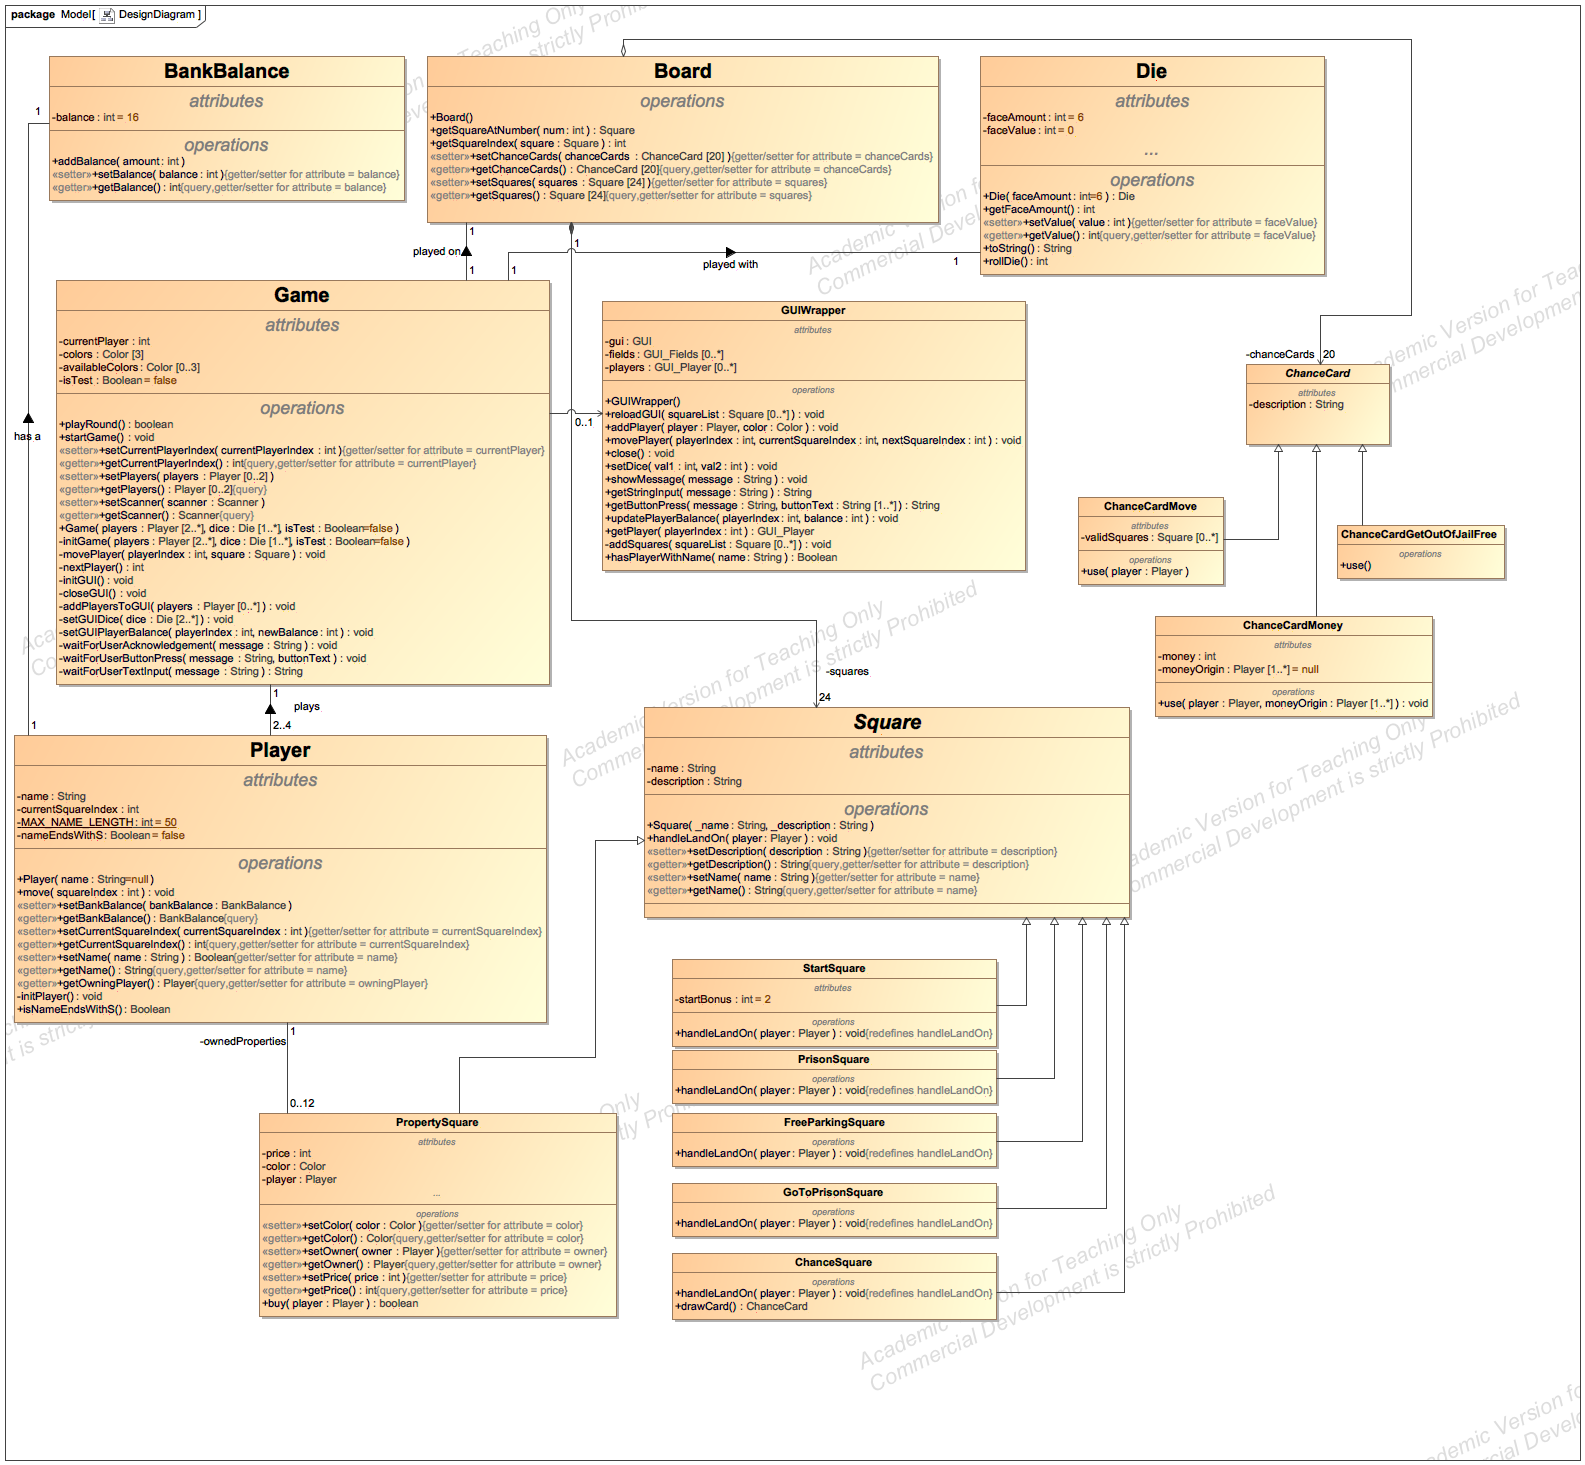
\includegraphics[width=0.8\textheight]{figures/DesignDiagram.png}}
    \caption{Designklassediagram\newline }
    
    \label{fig:designclass_diagram}
\end{figure}

\newpage 

% GRASP-principper i designklassediagram
\subsubsection{GRASP principper for designklassediagram}
\TODO (Kan ændres i forhold til klassediagrammet)

\begin{itemize}
    \item Creator: 
    \begin{itemize}
        \item  \textit{Board} er ansvarlig for at indeholde objekter af \textit{Square} og aggregerer \textit{ChanceCard} objekter
        \item  \textit{Player} har til ansvar at benytte objekter af \textit{BankBalance} og kan indeholde \textit{PropertySquare} objekter
        \item \textit{Square}s ansvarsområde omhandler indholdet af objekter fra \textit{PropertySquare}, \textit{StartSquare}, \textit{PrisonSquare}, \textit{FreeParkingSquare}, \textit{GoToPrisonSquare} og \textit{ChanceSquare}
        \item \textit{Game} har samme mængde ansvar som i CDIO2
    \end{itemize}
    \item Information Expert: (Fra Game til Square er det næsten det samme som i CDIO2)
    \begin{itemize}
        \item Klassen \textit{Game} er en information expert, der står for at håndtere spiller og at spillerne rykkes rundt på spillepladen
        \item \textit{BankBalance}-klassen har informationerne til at ændre spillerens pengebeholdning
        \item \textit{Board}-klassen er en information expert, som håndterer felter, der er givet ved navn og beskrivelse
        \item \textit{Square}-klassen har infomationer til at skabe et felt med navn og beskrivelse
        \item \textit{PropertySquare} indeholder informationer til at generere et felt bestående af pris, farve og ejerskab
    \end{itemize}
    \item Low Coupling:
    \begin{itemize}
        \item Der er hovedsageligt få koblinger mellem klasserne, hvor den største mængde koblinger er 7 på klassen \textit{Square}
        \item Da \textit{Square} har mange koblinger, støtter den ikke low coupling, men klassen har stadig high cohesion
    \end{itemize}
    \item High Cohesion:
    \begin{itemize}
        \item Generelt er der tale om high cohesion mellem klasserne, da de har en passende mængde ansvar for kodegenerering som opfyldes ved samarbejde med andre klasser
        \item \TODO !!(Hvis der opstår problemer med implementering, kan det skyldes low cohesion)!! Notice
    \end{itemize}
    \item Controller: (Kopieret fra CDIO2)
    \begin{itemize}
        \item Klassen \textit{Game} vælges som facade controller, som står for inputs til systemet. Det skyldes at \textit{Game} ikke vurderes at have så stort ansvar, at den bliver incohesive
    \end{itemize}
\end{itemize}



% Sekvensdiagram
\subsection{Sekvensdiagram }

\TODO Intro sekvensdiagram


%Sekvensdiagram for ....?
\subsubsection{Kast af terning}
\TODO Someone please fix
%\begin{figure}[H]
%    \centering
%   {\includegraphics[width=0.5\textheight]{figures/}}
%    %\includegraphics[width=0.6\linewidth]{figures/}
%    \caption{Sekvensdiagram over ...}
%    \label{fig:sekvensdia1}
%\end{figure}
\begin{figure}[H]
    \centering
    \includegraphics[width=0.7\linewidth]{figures/sekvensDiagrammer/KastTerningSekvensDiagram.png}
    \caption{Sekvensdiagram over kast af terning \TODO Skal det være use-case ID}
    \label{fig:sekvensKastTerning}
\end{figure}

%Pakkediagram? (Måske)
\subsection{Pakkediagram (Måske?) }
\TODO{Afhænger måske af om det var rigtigt sidst, for så er det meget nemt at lave.}

\end{flushleft}
\end{document}
